\documentclass[xcolor=table]{beamer}
\usepackage[utf8]{inputenc}
\usepackage[italian]{babel}

\usetheme{Frankfurt} % Darmstadt, Frankfurt.
\beamertemplatenavigationsymbolsempty % Temove navigation symbols.

% Images.
\usepackage{graphicx}
\usepackage{multicol}

% Code.
\usepackage{listings}

% Math.
\usepackage{siunitx}

\title
{High Level Synthesis of a trained CNN for handwritten digit recognition}

%\subtitle{Past, present, and future}
\institute
{
  \large{Embedded Systems}
  \newline
  \small{Università degli Studi di Parma}
}

\author{
  Federico Serafini
  \newline
  \small\texttt{federico.serafini@studenti.unipr.it}
}

\date{12/07/2022}

%%%%%%%%%%%%%%%%%%%%%%%%%%%%%%%%%%%%%%%%%%%%%%%%%%%%%%%%%%%%%%%%%%%%%
\begin{document}

% Title page.
\begin{frame}[plain] % Remove outline bar on top.
  \titlepage
\end{frame}

\begin{frame}{Outline}
  \tableofcontents
\end{frame}

\section{Introduction}

\begin{frame}{Basic concepts}
  \begin{block}{Convolutional Neural Network (CNN)}
    Neural network with a special architecture that is able to detect spatial structures (features) of the input:
    \begin{itemize}
      \item widely used in image-recongnition problems;
      \item highly-parallelizable algorithm.
    \end{itemize}
  \end{block}

  \centering
  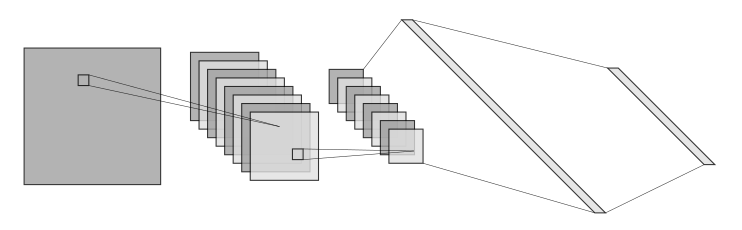
\includegraphics[scale=0.42]{Images/cnn.png}
\end{frame}

\begin{frame}{Basic concepts}
  \begin{block}{A single and abitious objective}
    Overtake C performances through HW parallelism!
  \end{block}
  \begin{block}{Workflow}
    \begin{enumerate}
      \item
        Python:
        \begin{enumerate}
          \item
            model definition, training and evaluation;
          \item
            export of (trained) network weights and architecture.
        \end{enumerate}
      \item
        C: replication of the network.
      \item
        Vitis HLS:
        \begin{enumerate}
          \item
            naive approach (high level synthesis of basic C);
          \item
            stream and dataflow approach.
        \end{enumerate}
      \item
        Verification.
    \end{enumerate}
  \end{block}
\end{frame}

\section{SW Implementation}

\begin{frame}{Model definition and evaluation in Python}
  \begin{columns}[T]
    \begin{column}{0.45\columnwidth}
      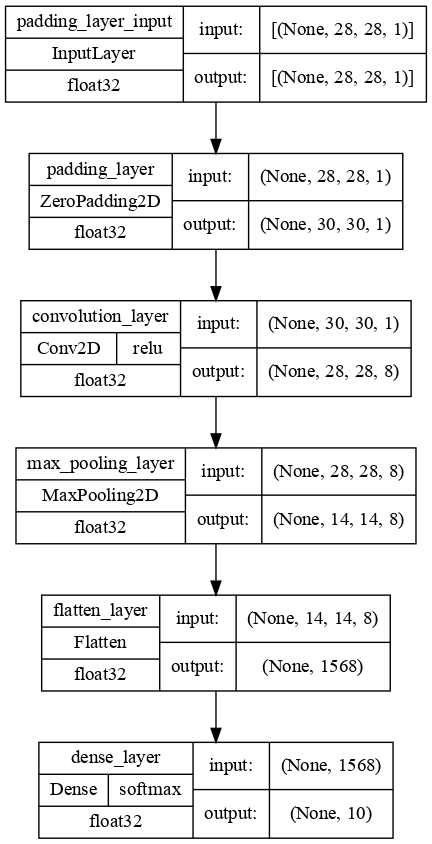
\includegraphics[scale=0.25]{Images/model.png}
    \end{column}
    \begin{column}{0.3\columnwidth}
      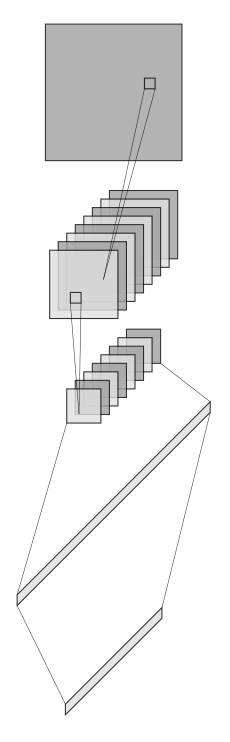
\includegraphics[scale=0.3]{Images/cnn-vertical.png}
    \end{column}
    \begin{column}{0.5\columnwidth}
      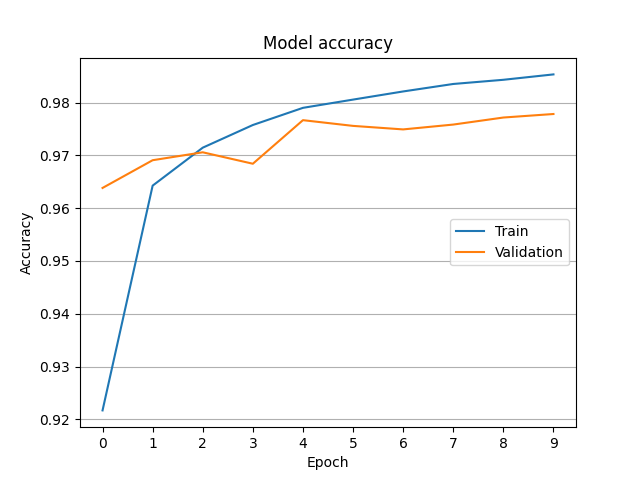
\includegraphics[scale=0.3]{Images/accuracy.png}
      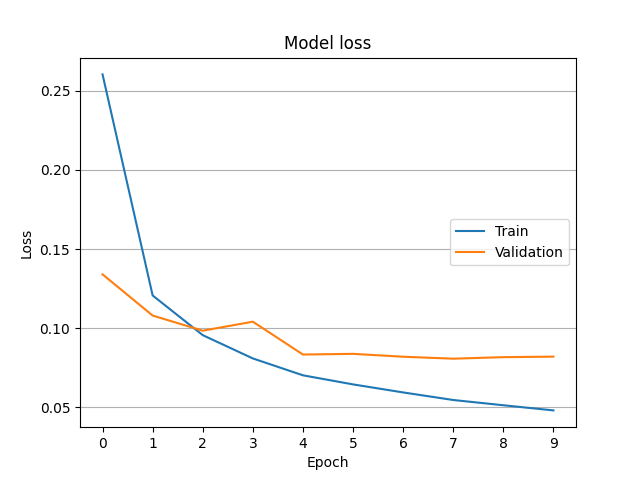
\includegraphics[scale=0.3]{Images/loss.png}
    \end{column}
  \end{columns}
\end{frame}

\definecolor{green}{rgb}{0, 0.6, 0}

\begin{frame}[fragile]{Network replication in C}
  \begin{lstlisting} [language=C, basicstyle=\tiny\ttfamily, numbers=left, commentstyle=\color{green}]
void cnn
(
  float img_in     [IMG_ROWS][IMG_COLS],
  float prediction [DIGITS]
)
{
  /******** Normalization and padding. ********/
  float pad_img [PAD_IMG_ROWS][PAD_IMG_COLS] = { 0 };
  normalization_and_padding(img_in, pad_img);

  /******** Convolution layer. ********/
  float features [FILTERS][IMG_ROWS][IMG_COLS] = { 0 };
  // Convolution with relu as activation function.
  convolutional_layer(pad_img, features);

  /******** Max-pooling layer. ********/
  float pool_features [FILTERS][POOL_IMG_ROWS][POOL_IMG_COLS] = { 0 };
  max_pooling_layer(features, pool_features);

  /******** Flatten layer. ********/
  float flat_array [FLAT_SIZE] = { 0 };
  flattening_layer(pool_features, flat_array);

  /******** Dense layer. ********/
  dense_layer(flat_array, prediction);
}
  \end{lstlisting}
\end{frame}

\section{High Level Synthesis}

\begin{frame}{Naive approach: latency estimation}
\centering
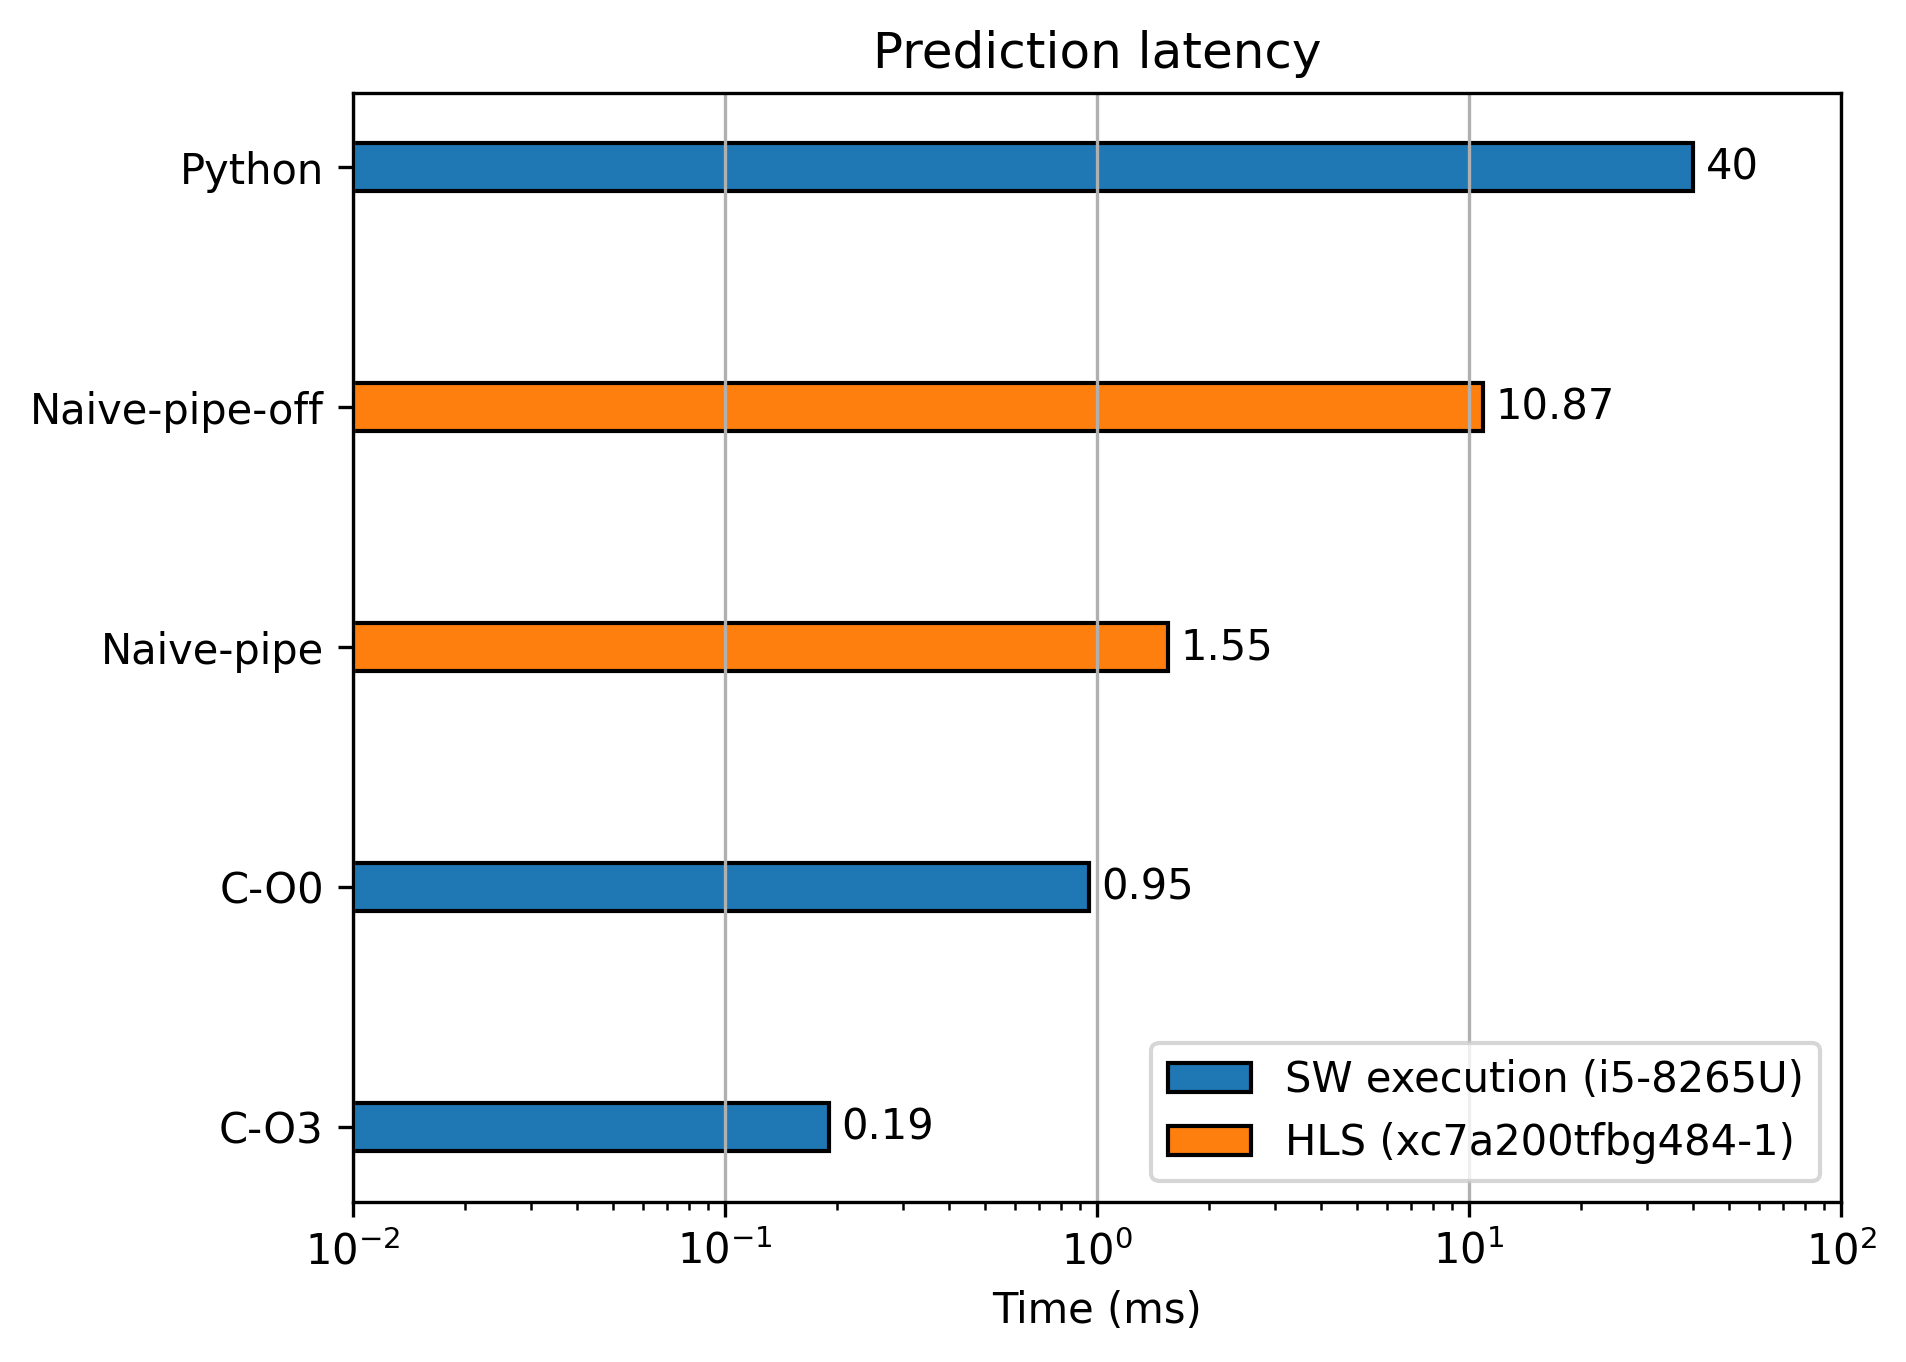
\includegraphics[scale=0.65]{Images/early-plot.png}
\end{frame}

\begin{frame}{Vitis HLS Stream
  \footnote{
    \href{https://docs.xilinx.com/r/en-US/ug1399-vitis-hls/HLS-Stream-Library}
    {Vitis-HLS User Guide}
  }
}
  \begin{block}{Streaming data transfer}
     \begin{itemize}
       \item
       A FIFO queue (\emph{ap\_fifo} interface).
       \item
       Data samples are sent in sequential order
       starting from the first (no address management is required).
     \end{itemize}
  \end{block}
  \begin{block}{Array implemented as FIFO interface}
    \begin{itemize}
      \item[\textcolor{orange}{\textbullet}]
      Array must be only read or written, thus allowing a point-to-point
      connection.
      \item[\textcolor{orange}{\textbullet}]
      Program must follow a FIFO semantics (no random accesses).
      \item[\textcolor{green}{\textbullet}]
      If a stream is used to transfer data between tasks, consider a dataflow region where data streams from one task to the next.
    \end{itemize}
  \end{block}
\end{frame}

\begin{frame}[fragile]{Stream-dataflow approach: code structure}
  \begin{lstlisting} [language=C, basicstyle=\tiny\ttfamily, numbers=left, commentstyle=\color{green}]
#define FILTERS 8

void cnn
(
  float img_in     [IMG_ROWS][IMG_COLS],
  float prediction [DIGITS]
)
{
  /******** Pre-processing the img_in. ********/

  // Normalization and padding.

  /******** Clone the normalized and padded image. ********/

  /*
   *  Clone the normalized and padded image in order to
   *  have an image for each parallel execution (for each filter).
   */

  /******** Parallel executions start here. *********/

  /*  Dataflow section with streams used to transfer data between tasks:
   *  -convolution_layer;
   *  -max_pooling_layer;
   *  -flattening_layer;
   *  -dense_layer;
   *  -dense_layer_softmax.
   */
}
  \end{lstlisting}
\end{frame}

\begin{frame}{Dataflow view}
  \centering
  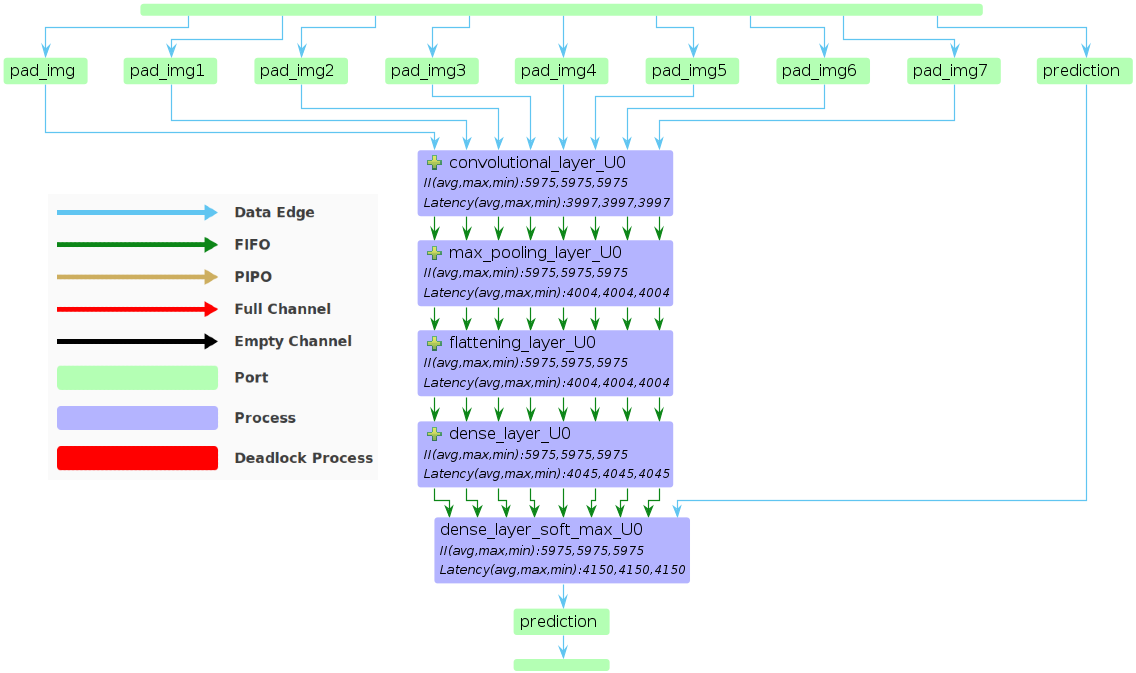
\includegraphics[scale=0.29]{Images/dataflow-and-legend.png}
\end{frame}

\section{Results and Verification}

%\begin{frame}{High level synthesis details report}
%  \centering
%  \small\text{`cnn' report}
%  \begin{figure}[H]
%    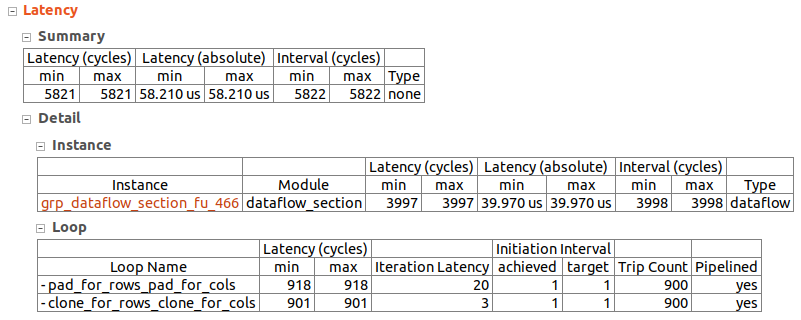
\includegraphics[scale=0.305]{Images/cnn-latency.png}
%  \end{figure}
%  \centering
%  \small\text{`dataflow\_section' report}
%  \begin{figure}
%    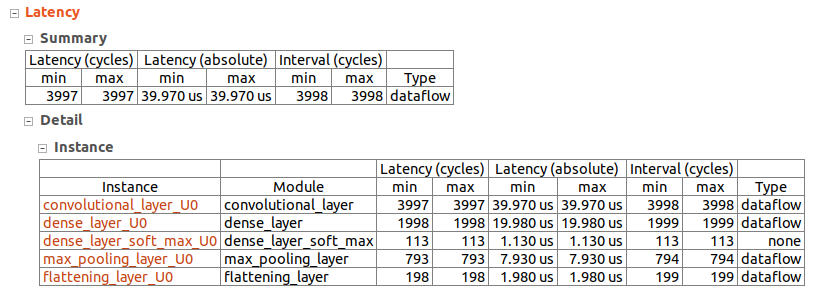
\includegraphics[scale=0.305]{Images/dataflow-latency.png}
%  \end{figure}
%\end{frame}

\begin{frame}{Stream-dataflow approach: latency estimation}
  \centering
  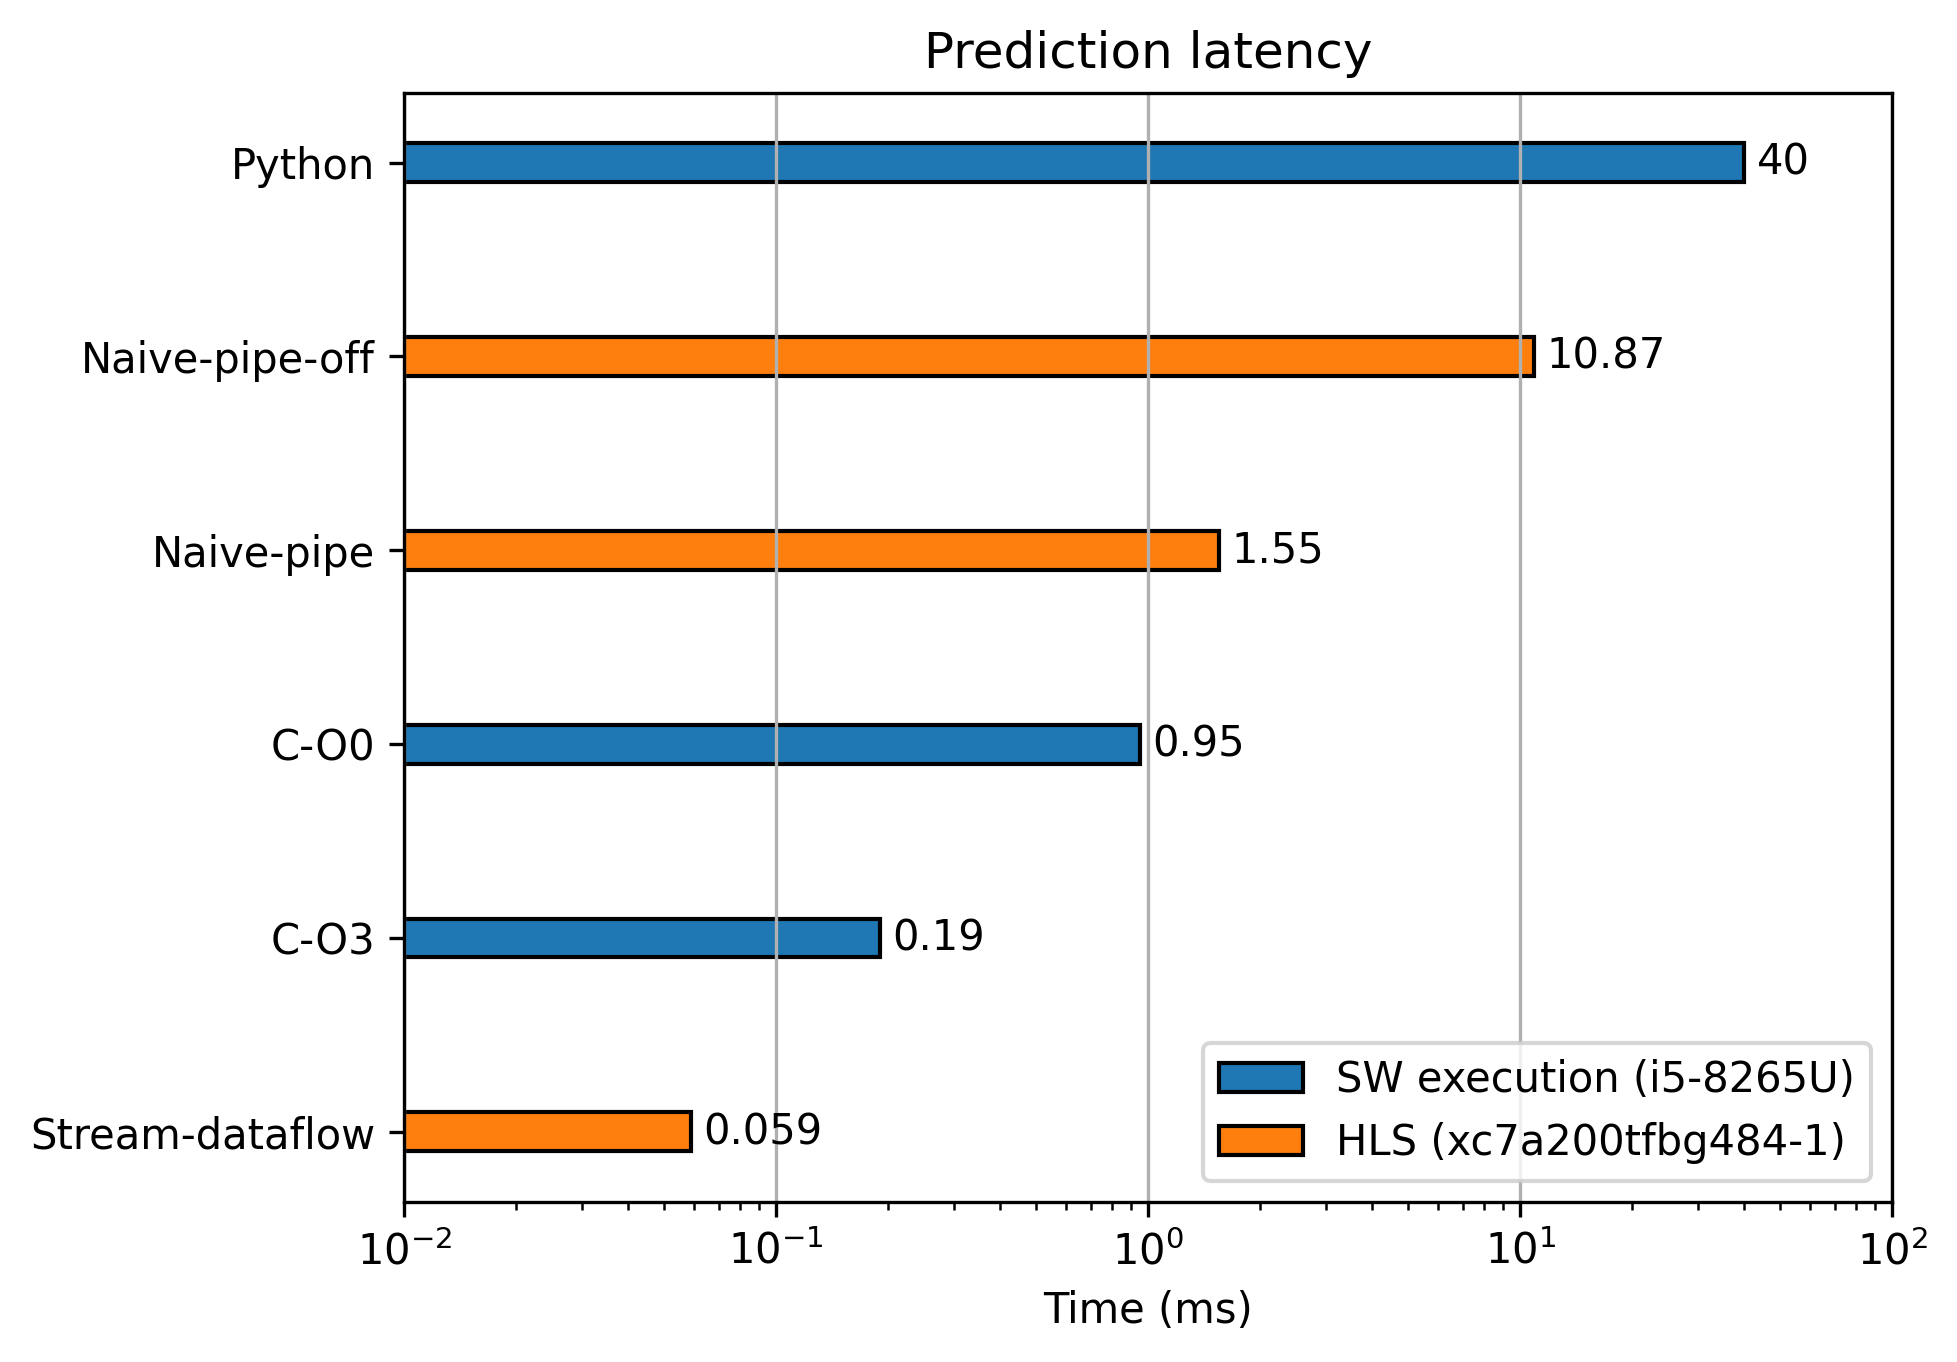
\includegraphics[scale=0.65]{Images/final-plot.png}
\end{frame}

\begin{frame}{Verification}
  \begin{block}{Co-simulation}
        \begin{table}
          \flushleft
          \begin{tabular}{|c|c|}
            \hline
            \pmb{Total predictions} & 10 \\
            \hline
            \pmb{Correct predictions} & 100\% \\
            \hline
          \end{tabular}
        \end{table}
        \begin{table}
          \flushleft
          \begin{tabular}{|c|c|c|c|}
            \hline
            &\pmb{Min} &\pmb{Avg} &\pmb{Max}\\
            \hline
            \pmb{Latency (cycles)}
            & 5975
            & 5975
            & 5975 \\
            \hline
          \end{tabular}
        \end{table}
  \end{block}
  \begin{block}{Export RTL with Vivado synsthesis and place and route}
    \begin{table}
      \flushleft
      \begin{tabular}{|c|c|c|c|c|}
        \hline
        &\pmb{BRAM} &\pmb{DSP}& \pmb{FF} &\pmb{LUT}\\
        \hline
        \pmb{Vitis HLS}
        &384
        &143
        &47201
        &37585 \\
        \hline
        \pmb{Vivado}
        &224
        &143
        &38791
        &26753\\
        \hline
      \end{tabular}
    \end{table}
    \begin{table}[H]
      \flushleft
      \begin{tabular}{|c|c|c|c|}
        \hline
        &\pmb{Required} &\pmb{Post-synth} &\pmb{Post-impl}\\
        \hline
        \pmb{Clock period (\unit{\nano\second})}
        &10
        &8.123
        &9.157\\
        \hline
      \end{tabular}
    \end{table}
  \end{block}
\end{frame}

\section{Conclusions}

\begin{frame}{Conclusions and future work}
  \begin{block}{Future work}
    \begin{itemize}
      \item Smarter SW algorithm $\longrightarrow$ smarter HW accelerator.
      \item Fixed-point arithmetic $\longrightarrow$ reduced area.
      \item Vitis HLS syntax constructs and libraries $\longrightarrow$ better synthesis.
    \end{itemize}
  \end{block}

  \begin{block}{Hardware or software implementation?}
    Further invistigation is needed:
    \begin{enumerate}
      \item
      apply improvements listed above;
      \item
      consider application domain requirements (for example the available HW and timing constraints);
      \item
      consider also a co-design (HW and SW);
      \item
      choose the cheapest solution satisfying the requirements.
    \end{enumerate}
  \end{block}
\end{frame}

\begin{frame}[plain]
  \centering
  \huge Thank you for your attention.
\end{frame}

\end{document}